\section{Användargränssnitt}
QuadOpt använder sig av två olika typer av gränssnitt för att man ska kunna skicka in optimeringsproblemet till lösaren.

\subsection{MATLAB}
I MATLAB kommer QuadOpt kunna köras direkt via funktionsanropet

\begin{lstlisting}
z = quadopt(Q, q, E, h, F, g, iter, time);
\end{lstlisting}

\begin{itemize}
	\item z - Matris där lösningen sparas.
	\item Q - Matris innehållande den kvadratiska delen av problemet.
	\item q - Matris innehållande den linjära delen av problemet.
	\item E - Ekvivalensbivillkorsmatrisen.
	\item h - Ekvivalensbivillkoren i högerledet.
	\item F - Olikhetsbivillkorsmatrisen (\textbf{OBS!} det är större än eller lika med g).
	\item g - Olikhetsbivillkoren i högerledet.
	\item iter - Max antal iterationer innan lösaren avbryter.
	\item time - Max tid i mikrosekunder innan lösaren avbryter.
\end{itemize}
Funktionen installeras i MATLAB genom att bygga en mex-fil som innehåller C-koden för konvertering av datastrukturer mellan MATLAB och QuadOpt. Det beräknade resultatet returneras tillbaka från QuadOpt till MATLAB, för mer information om Matlabfilen se avsnitt~\ref{subsec:mex} på sidan~\pageref{subsec:mex}.

\subsection{GUI}
QuadOpt går även att köra direkt via ett grafiskt gränssnitt, om man t.ex. inte skulle ha tillgång till Matlab. Det grafiska gränssnittet är skrivit i Python och är testat för version 3.2.3 eller senare, det använder också Pythons egna inbyggda grafikbibliotek \emph{tkinter}. ''C code'' knappen genererar en C-fil som tillsammans med QuadOpt kan lösa det specifika angivna optimeringsproblemet i programmet.

\begin{figure}[h!]
	\begin{center}
		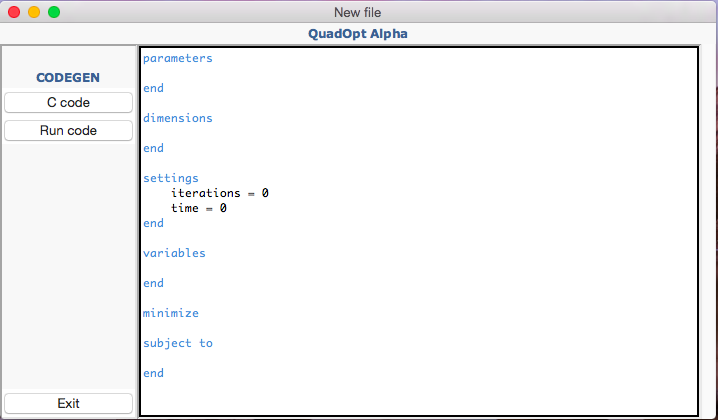
\includegraphics[scale=0.5]{bilder/macgui.png}
	\end{center}
	\caption{Användargränssnittet.}
\end{figure}

